\subsection{Probleme und Lösungen}
\subsubsection{Grenzen der Depth API und Occlusion}
\label{probleme-grenzen-depth-api}
Wie in Kapitel \ref{immersion} beschrieben trägt eine gute Verdeckung der virtuellen Objekte dazu bei, die Immersion in AR zu steigern\cite*[Breen et al. (1995)][]{breen1995}\cite*[Shah et al. (2012)][]{shah2012}. Umso wichtiger ist es, dass diese Funktion auch in dieser Anwendung gut funktioniert. Dabei gibt es drei Problematiken, die bei der Entwicklung in dieser Arbeit zum Vorschein kommen.

Das erste Problem ist, das diese API nicht für jedes Gerät verfügbar ist. Die Dokumentation von ARCore\cite*{ARCoreDokumentation} bietet eine Tabelle mit allen kompatiblen Geräten. Damit kann nicht sichergestellt werden, dass die Anwendung auf jedem Gerät gleich funktioniert. 

Ein weiteres Problem wird in Abbildung \ref*{fig:technische-umsetzung-arcore-depth-problem} deutlich. In diesem Beispiel wird Occlusion mit dem \textit{AR Occlusion Manager} implementiert, der an die \textit{AR Camera} angehängt wird. Die AR Camera wird in Kapitel \ref*{technische-umsetzung-platzierung-auf-einer-beliebigen-flaeche} erläutert. Das Beispiel ist vor Ort an einer Mauer vor dem Gebäude 4 aufgenommen. Das rote Quadrat ist die erzeugte Depth Map. Je dunkler die rote Farbe, desto näher ist das Objekt zur Kamera. Es wird deutlich, dass erst ab einer Entfernung von 1m überhaupt Tiefe erkannt wird. Aus einer Entfernung ab 1,5m wird keine Tiefe mehr erkannt. Dies ist insbesondere für AR im Freien problematisch. 

\begin{figure}[H]
    \centering
    \subfloat[][]{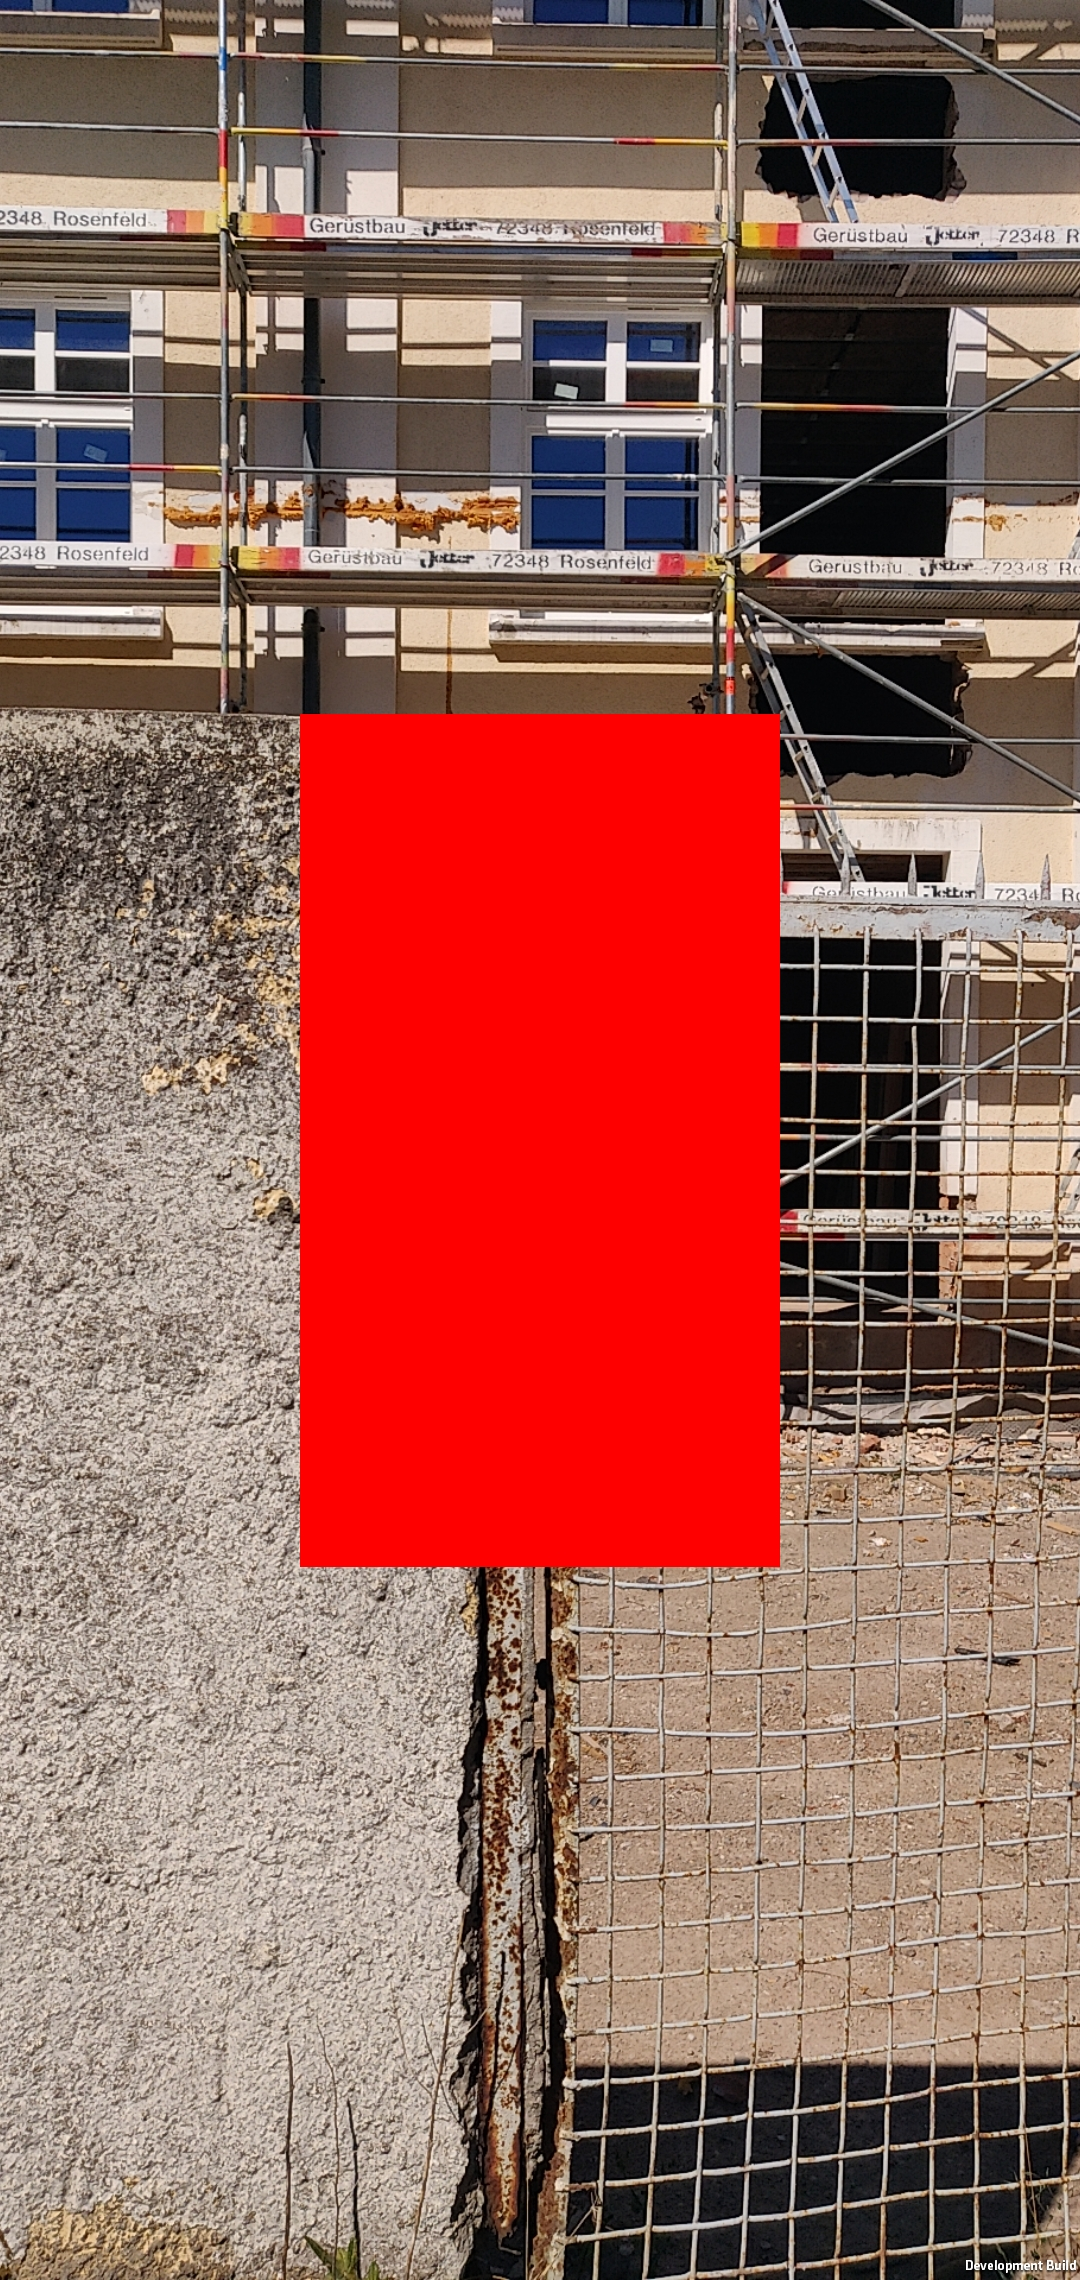
\includegraphics[width=0.3\linewidth]{img/anwendung/arcore/arcore-depth-occlusion.jpg}}%
    \qquad
    \subfloat[][]{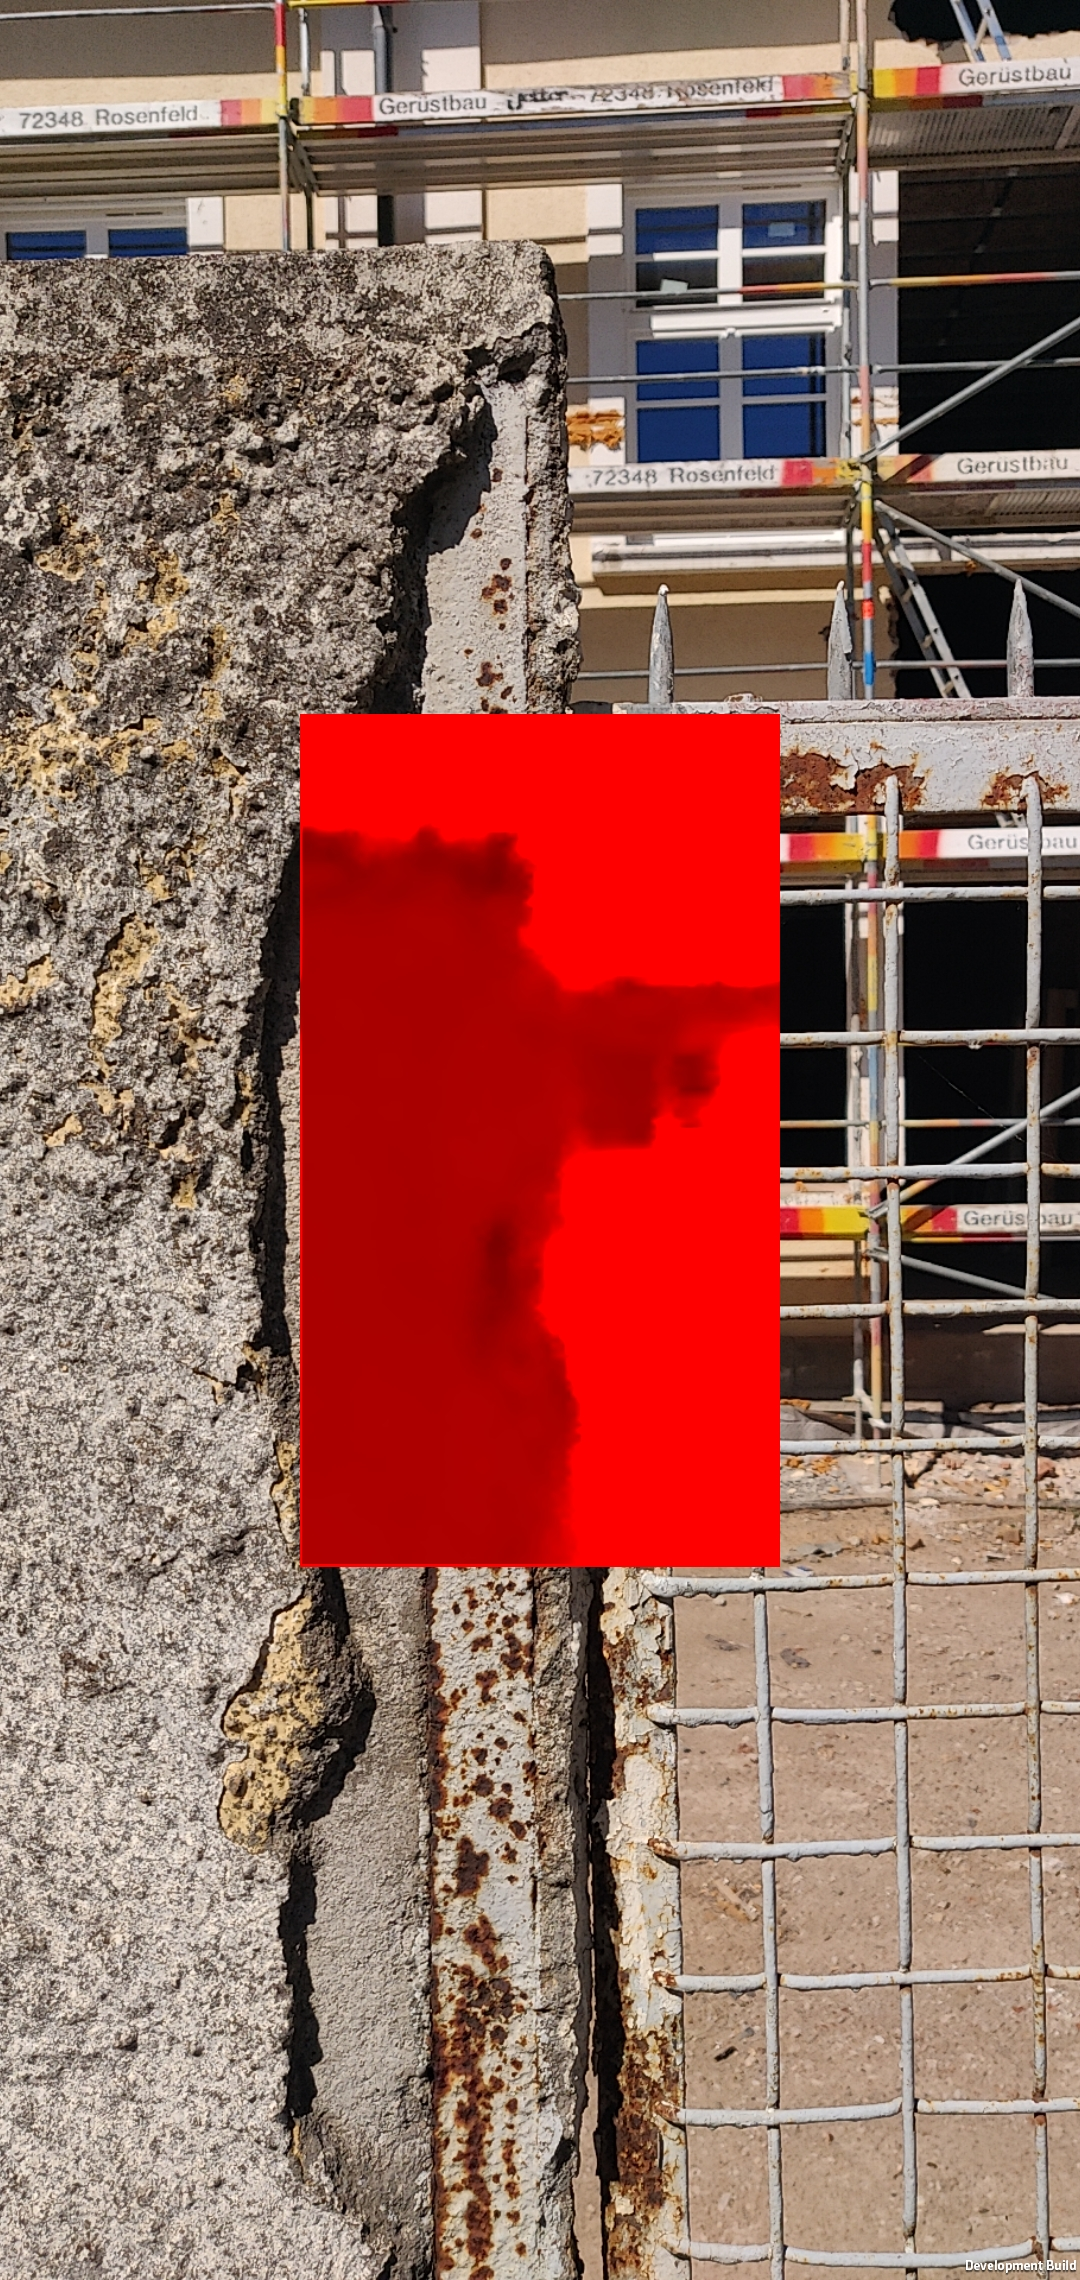
\includegraphics[width=0.3\linewidth]{img/anwendung/arcore/arcore-depth-occlusion-2.jpg}}%
    \qquad
    \subfloat[][]{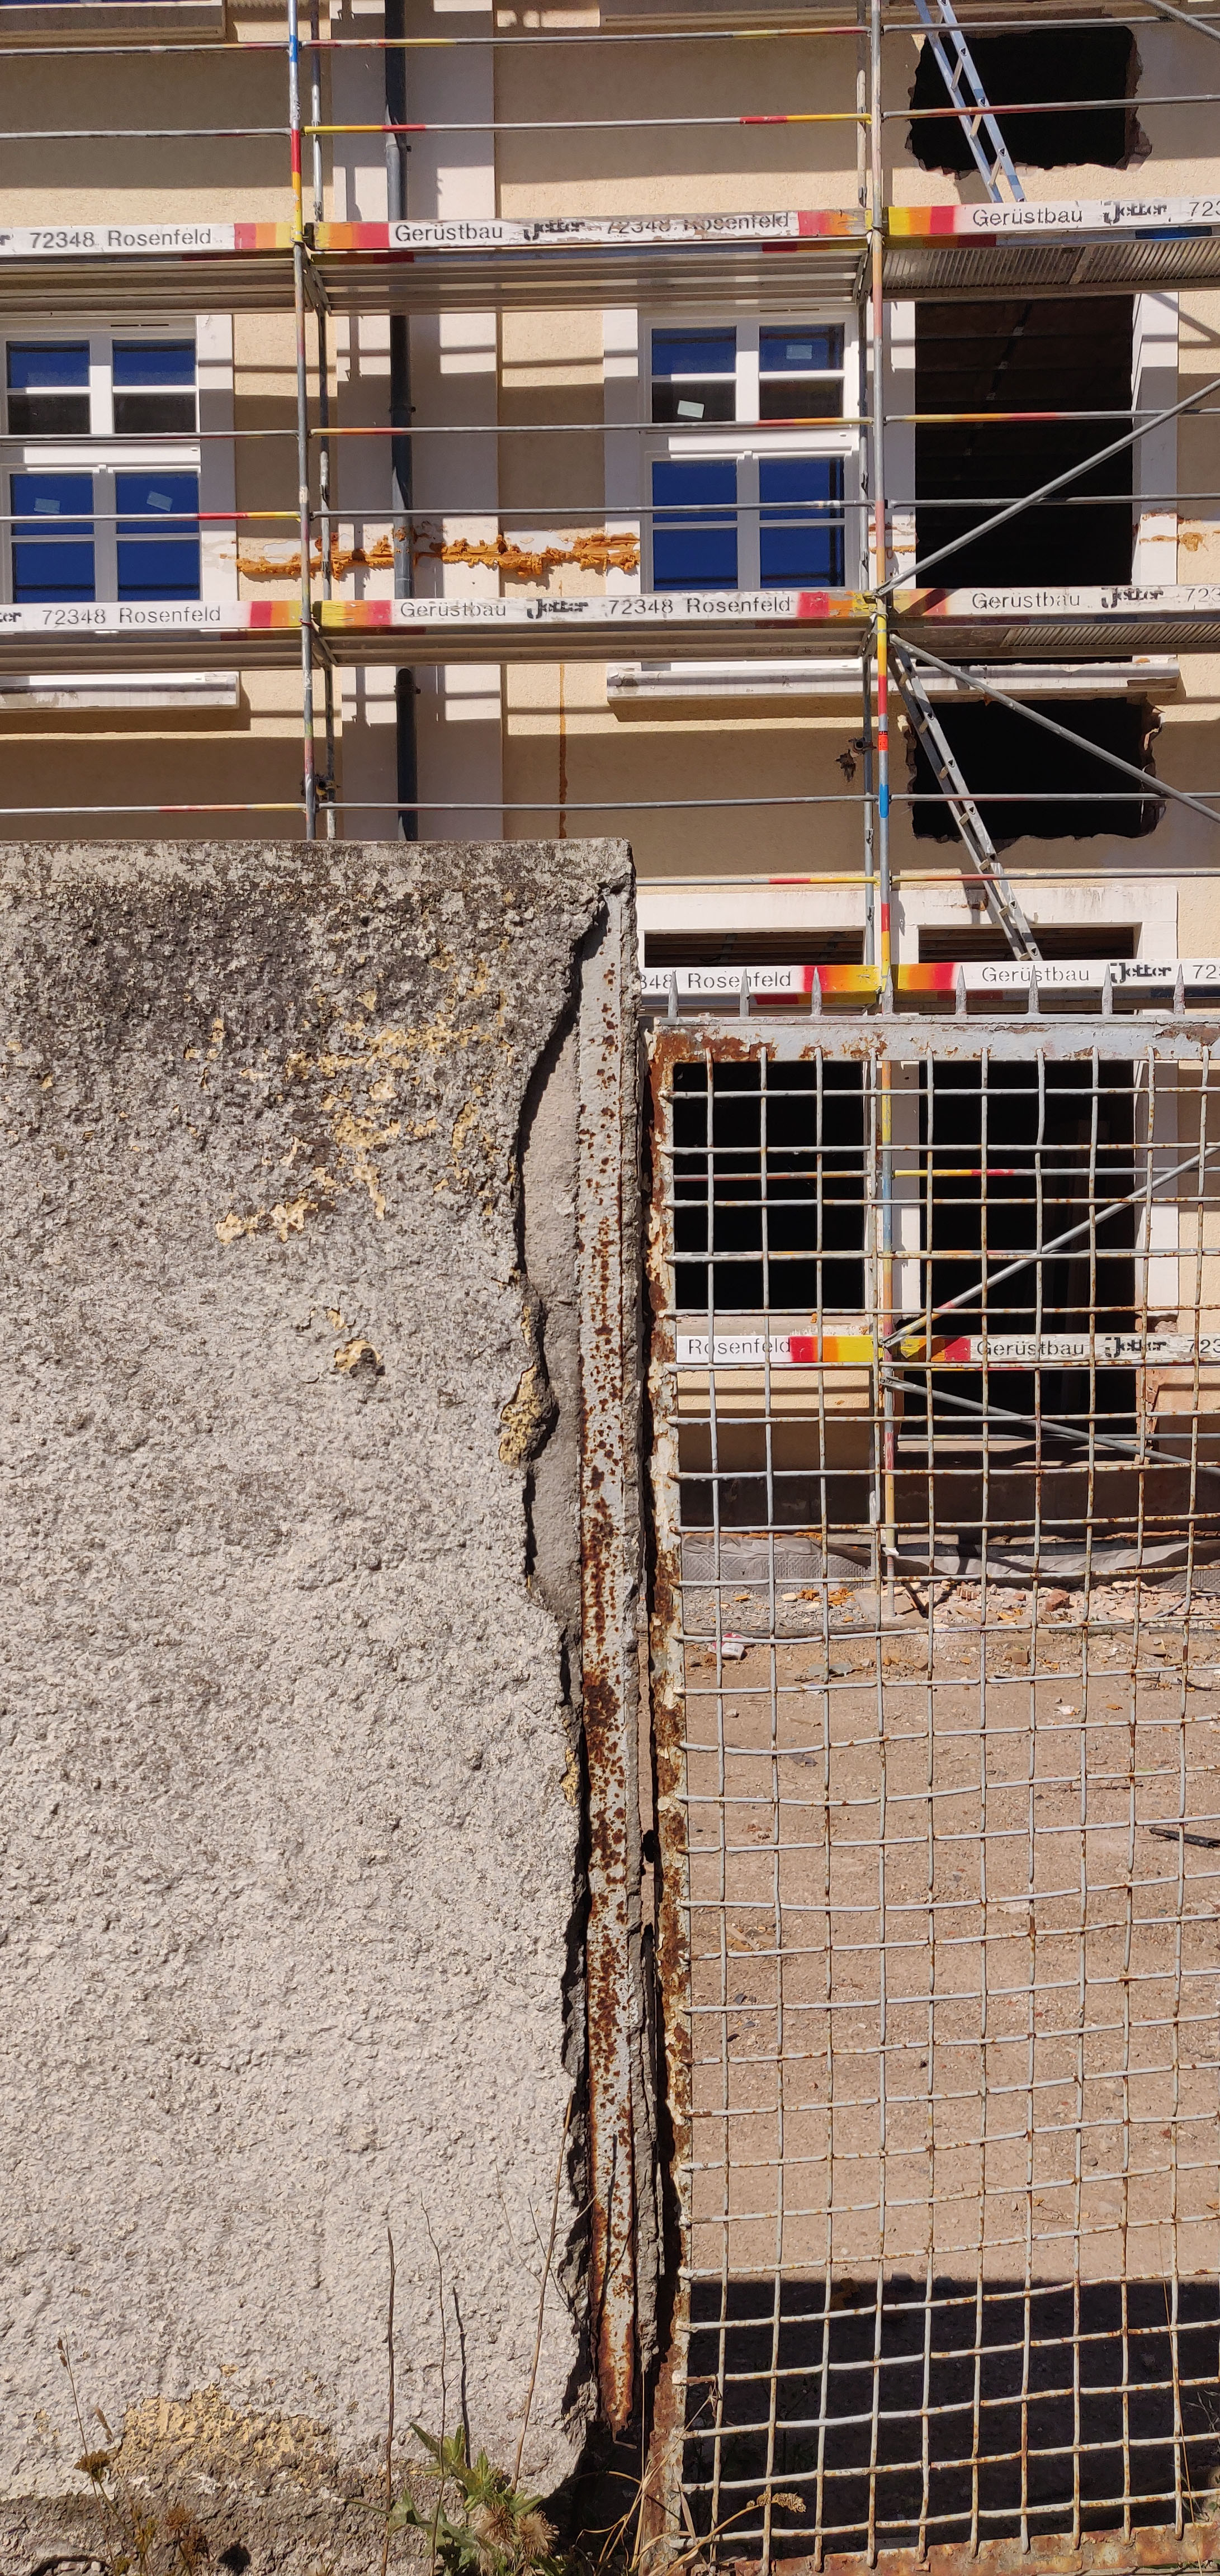
\includegraphics[width=0.3\linewidth]{img/anwendung/arcore/arcore-depth-occlusion-3.jpg}}%
    \qquad
    \caption{Die Depth Map aus einer Entfernung von 1,5m (a) im Vergleich zu der Depth Map aus 1m (b) und die Szene selbst mit der Mauer und dem Zaun aus 1,5m Entfernung(c).}%
    \label{fig:technische-umsetzung-arcore-depth-problem}
\end{figure}
% Ungenauigkeiten, auch auf andere Paper hinweisen
% GPS Experiment
% Vergleich Google Koordinaten und Vermessungsamt Koordinaten
In der Regel sind bei der Nutzung von GPS Positionsabweichungen von bis zu 10 Metern möglich. Eine genaue Platzierung der Gebäude ist daher problematisch.
% Abbildung mit Beispiel

Um die Tracking-Genauigkeit zu erhöhen, gibt es mehrere Methoden. \textit{DGPS (engl. Differential GPS)} verbessert GPS-Signale, indem es ein Korrektursignal durch eine ortsfeste Referenzstation mit bekannter Lokalisierung berechnet. Da es in Deutschland lediglich acht solcher Stationen gibt und einige Anbieter nur kommerziell die Daten bereitstellen, ist diese Methode nicht für diese Arbeit geeignet\footnote{https://www.heise.de/newsticker/meldung/Differential-GPS-und-WLAN-RTT-Praezise-Ortung-mit-Android-P-4046935.html} \footnote{Liste von DGPS-Sendern: https://www.ndblist.info/datamodes/worldDGPSdatabase.pdf}. Eine weitere bekannte Möglichkeit bietet \textit{SBAS (engl. Satellite Based Augmentation System)}, bei dem mehrere geostationäre Satelliten das GPS Signal auf bis zu einem Meter Genauigkeit zu verbessern \cite*{doerner}.

Platinsky et al.\cite{platinsky} erstellen für ein besseres Tracking bei fehlender GPS Genauigkeit ein 3D-Modell der Umgebung. Bei der anschließenden AR Nutzung in diesem Gebiet wird auf dem Smartphone SLAM betrieben. Die Daten vom Smartphone werden mit der 3D-Karte verglichen, um ein genaueres Tracking durchzuführen.